\documentclass[tikz,border=10pt]{standalone}
\usepackage{tikz}
\usetikzlibrary{arrows.meta, positioning, shapes.geometric}

% Define colors
\definecolor{varcolor}{RGB}{190,220,245}
\definecolor{constraintcolor}{RGB}{255,215,170}
\definecolor{expressioncolor}{RGB}{200,235,195}

\begin{document}

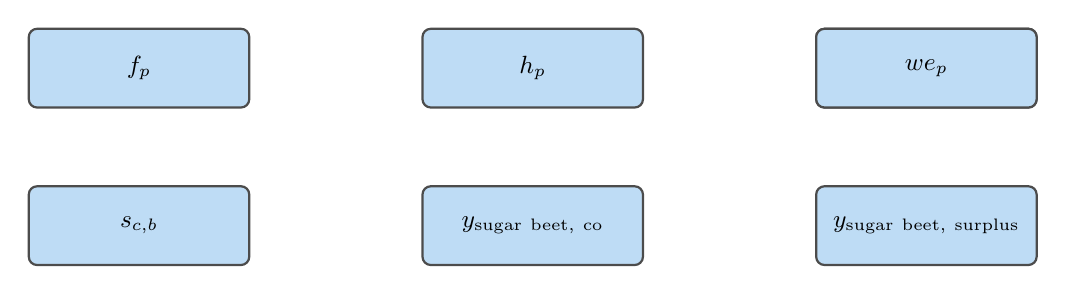
\begin{tikzpicture}[
    % Common block style
    block/.style={
        rectangle,
        rounded corners=3pt,
        draw=black!70,
        thick,
        minimum width=2.8cm,
        minimum height=1cm,
        align=center,
        font=\small
    },
    opt-var/.style={block, fill=varcolor},
    constraint/.style={block, fill=constraintcolor},
    expression/.style={block, fill=expressioncolor},
    arrow/.style={
        -{Stealth[length=2.5mm]},
        thick,
        draw=black!75
    },
    node distance=1.5cm and 1.8cm
]

% --- Variables ---
\node[opt-var] (share) at (0,0) {$\text{s}_{c,b}$};
\node[opt-var] (y-co) at (5,0) {$y_{\mathrm{sugar\ beet,\ co}}$} ;
\node[opt-var] (y-co) at (10,0) {$y_{\mathrm{sugar\ beet,\ surplus}}$};
\node[opt-var] (fh) at (0, 2) {$f_p$};
\node[opt-var] (hh) at (5, 2) {$h_p$};
\node[opt-var] (water-start) at (10, 2) {$ws_p$};
\node[opt-var] (water-end) at (10, 2) {$we_p$};



% --- Expressions ---


% --- Constraints ---


% --- Connections ---

\end{tikzpicture}

\end{document}

%%% Local Variables:
%%% mode: LaTeX
%%% TeX-master: t
%%% End:
